\documentclass{beamer}
\usetheme{Frankfurt}

\AtBeginSection[]
{
  \begin{frame}<beamer>
    \frametitle{\thesection}
    \tableofcontents[currentsection]
  \end{frame}
}

\title{Data Structures and Performance for Scientific Computing with Hadoop and Dumbo}
\author{Austin R. Benson \\
\vspace{0.2in}
Computer Sciences Division, UC-Berkeley \\
ICME, Stanford University}
\begin{document}
\maketitle

\section{Matrix storage}


\begin{frame}
\frametitle{Dense matrix storage}

\begin{center}
$A = \begin{pmatrix}
11 & 12 & 13 & 14 \\
21 & 22 & 23 & 24 \\
31 & 32 & 33 & 34 \\
41 & 42 & 42 & 44 \\
\end{pmatrix}$
\end{center}

\vspace{0.2in}

How do we store the matrix in HDFS?

\end{frame}

\begin{frame}
\frametitle{Dense matrix storage}

\begin{center}
$A = \begin{pmatrix}
11 & 12 & 13 & 14 \\
21 & 22 & 23 & 24 \\
31 & 32 & 33 & 34 \\
41 & 42 & 42 & 44 \\
\end{pmatrix}$
\end{center}

\vspace{0.2in}

In HDFS: 

\begin{center}

$\langle 1, [11,  12, 13, 14] \rangle$

\vspace{0.1in}

$\langle 2, [21, 22, 23, 24] \rangle$

\vspace{0.1in}

$\langle 3, [31, 32, 33, 34] \rangle$

\vspace{0.1in}

$\langle 4, [41, 42, 43, 44] \rangle$

\end{center}

\end{frame}



\begin{frame}
\frametitle{Two rows per record}

or we might use:

\begin{center}

$\langle 1, [ [11,  12, 13, 14], [21, 22, 23, 24] ] \rangle$

\vspace{0.1in}

$\langle 3, [[31, 32, 33, 34],[41, 42, 43, 44]] \rangle$

\end{center}

\end{frame}



\begin{frame}
\frametitle{Flattened list}

or maybe 

\begin{center}

$\langle 1, [11,  12, 13, 14, 21, 22, 23, 24 ] \rangle$

\vspace{0.1in}

$\langle 3, [31, 32, 33, 34, 41, 42, 43, 44] \rangle$

\end{center}

\vspace{0.2in}

... but we do lose information here (maybe it's not important)

\end{frame}

\begin{frame}
\frametitle{Full matrix}

or maybe 

\begin{center}

$\langle 1, [ [11,  12, 13, 14], [21, 22, 23, 24], [31, 32, 33, 34],[41, 42, 43, 44] ] \rangle$

\end{center}
\end{frame}


\begin{frame}
What is the "best" way?
\end{frame}

\begin{frame}
What is the "best" way? 

\vspace{0.2in}

Depends on the application... we will look at an example later.
\end{frame}


\section{Data}

\begin{frame}
\frametitle{Data Serialization}

\begin{center}
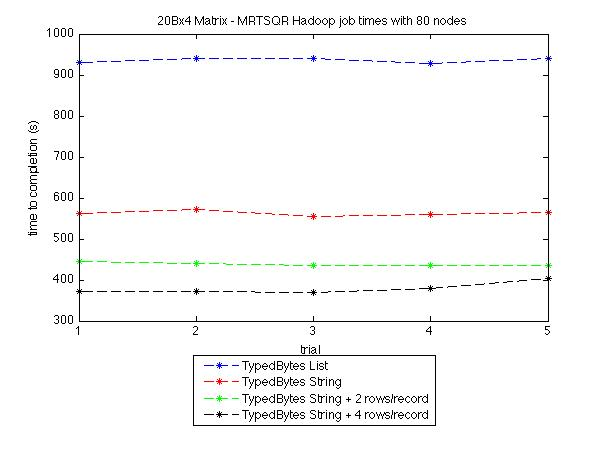
\includegraphics[height=2.in]{./images/A_20B_4_ser.jpg}
\end{center}

Small optimizations $\rightarrow$ 2.5x speedup!

\vspace{0.1in}

*all data from the NERSC Magellan cluster

\end{frame}

\begin{frame}
\frametitle{Data Serialization}

Same experiment but different matrix size (200 columns):

\begin{center}
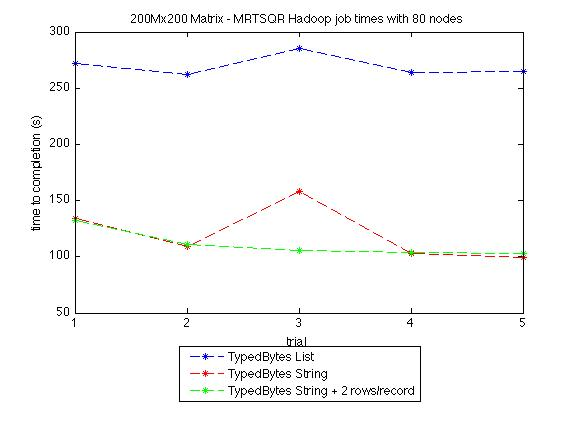
\includegraphics[height=2.in]{./images/A_200M_200_ser.jpg}
\end{center}

Again, 2.5x speedup!

\end{frame}

\begin{frame}
\frametitle{Languages}

Switching from Python to C++...

\begin{center}
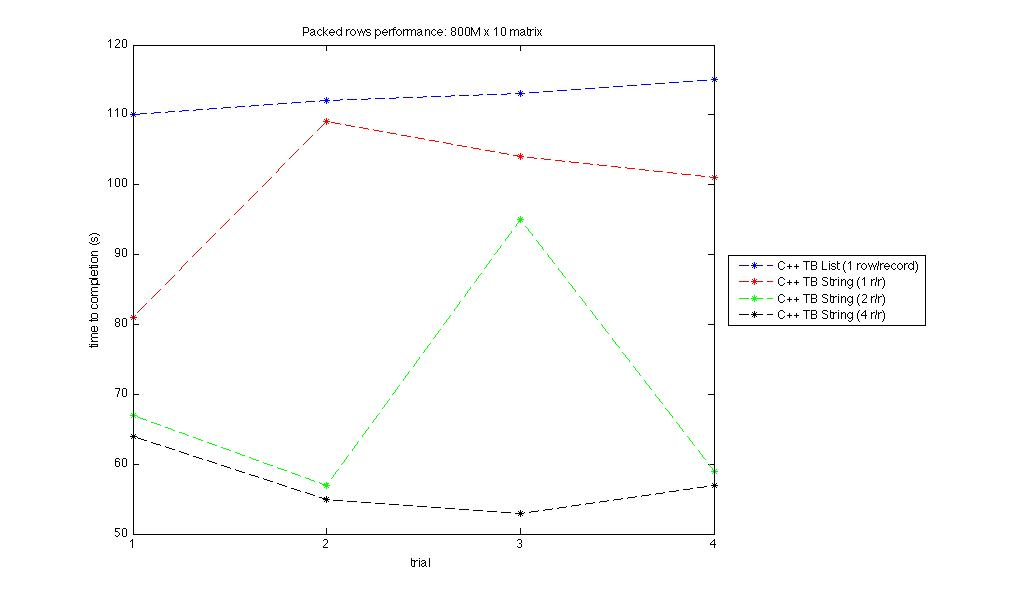
\includegraphics[height=2.in]{./images/cpp_perf.jpg}
\end{center}

same general trend

\end{frame}

\begin{frame}
\frametitle{More speedups}

Algorithm performance isn't the only place where we see speedups

\begin{center}
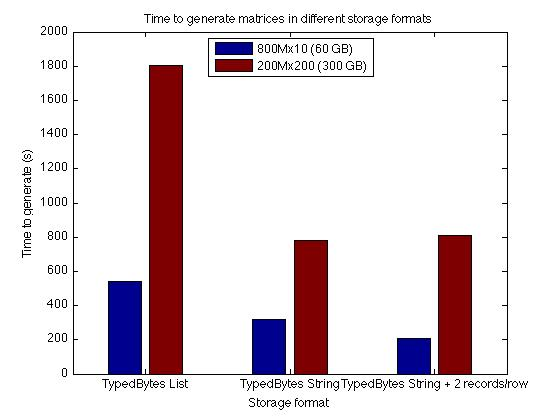
\includegraphics[height=2.in]{./images/gen_times.jpg}
\end{center}

\end{frame}


\begin{frame}

Why can we expect these speedups?

\begin{center}
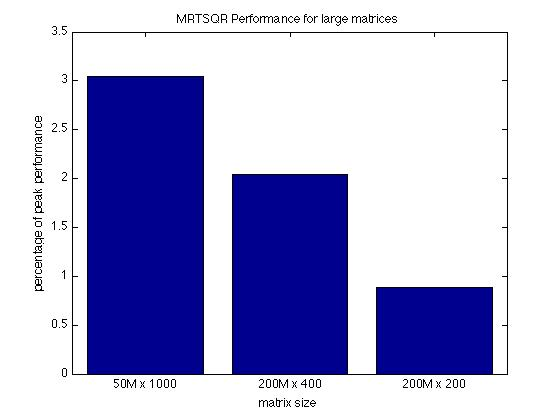
\includegraphics[height=2.in]{./images/peak_perf.jpg}
\end{center}

These are \emph{not} high-performance implementations.  We care about I/O performance.

\end{frame}

\section{Example: outputting many small matrices}

\begin{frame}

Suppose we need to write many small matrices to disk.

\begin{center}
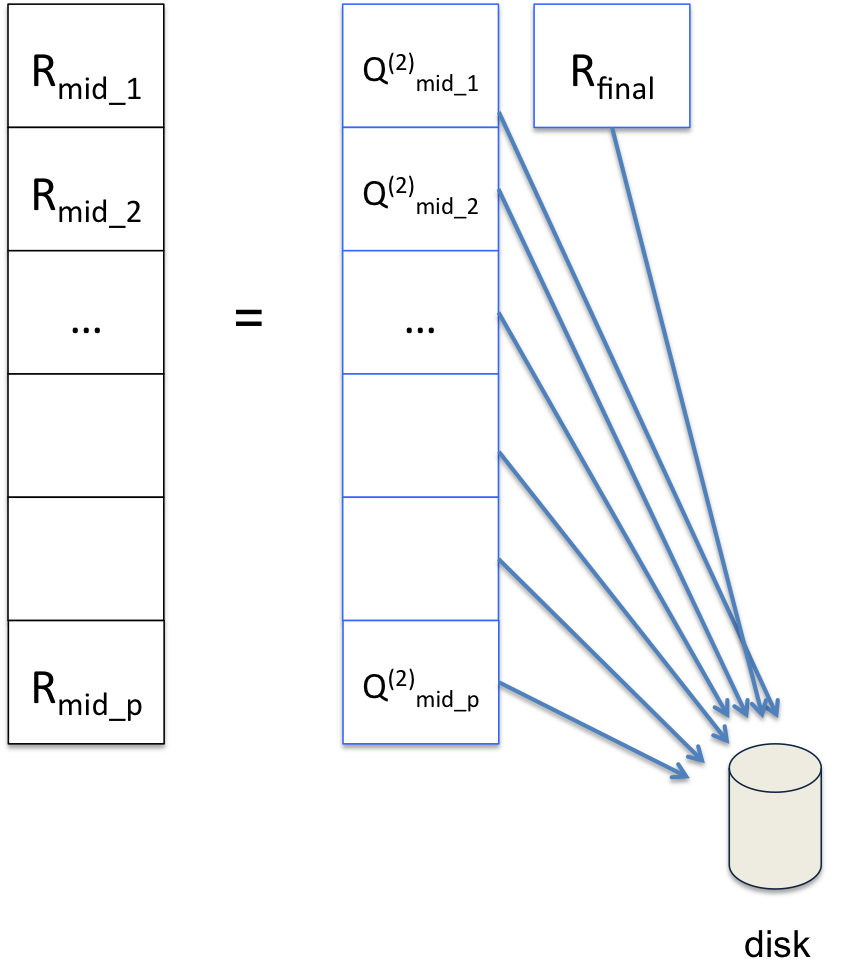
\includegraphics[height=2.in]{./images/full_2.png}
\end{center}

\end{frame}


\begin{frame}
\frametitle{Code}

Code: 

\vspace{0.2in}

git clone git://github.com/icme/mapreduce-workshop.git

cd mapreduce-workshop/arbenson

\vspace{0.2in}

Files:

\begin{itemize}
\item{speed\_test.py (tester)}
\item{small\_matrix\_test.py (driver)}
\end{itemize}


\end{frame}



\begin{frame}

\begin{center}
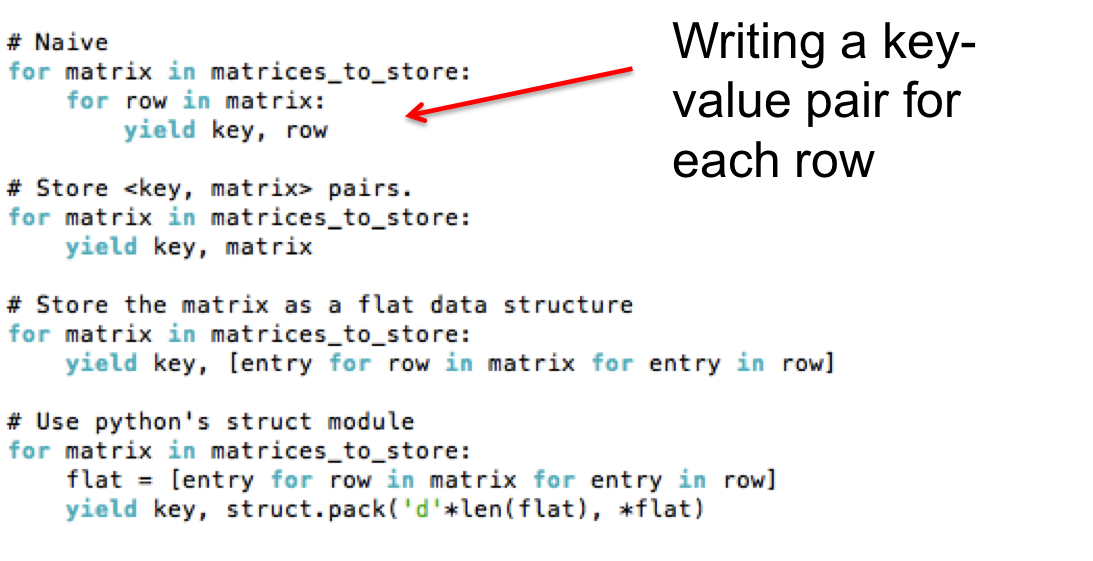
\includegraphics[height=2.in]{./images/small1.png}
\end{center}

\end{frame}

\begin{frame}

\begin{center}
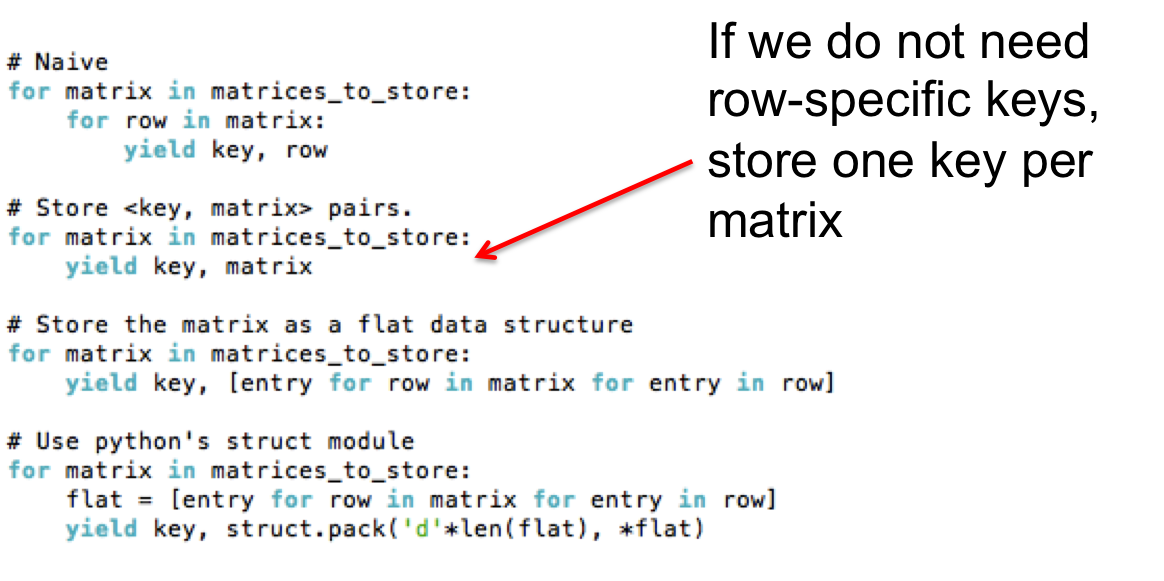
\includegraphics[height=2.in]{./images/small2.png}
\end{center}

\end{frame}

\begin{frame}

\begin{center}
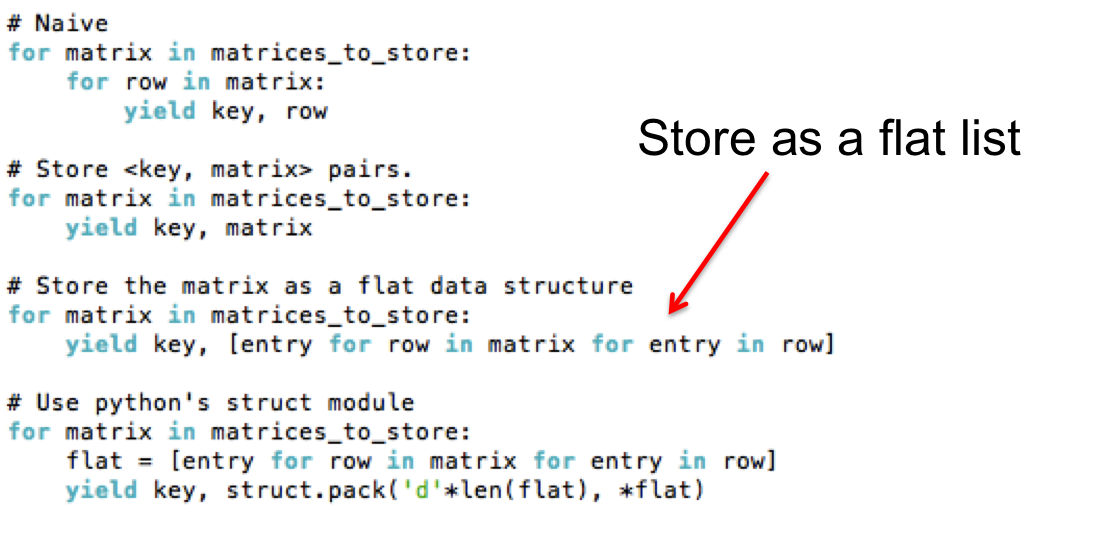
\includegraphics[height=2.in]{./images/small3.png}
\end{center}

\end{frame}

\begin{frame}

\begin{center}
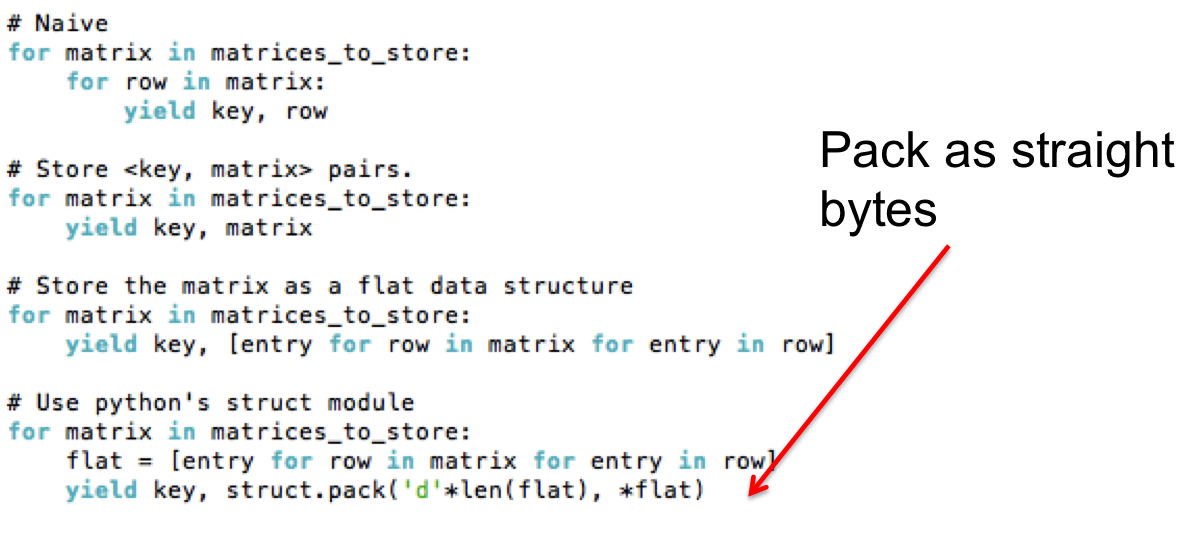
\includegraphics[height=2.in]{./images/small4.png}
\end{center}

\end{frame}

\section{Example: Cholesky QR}

\begin{frame}
\frametitle{Algorithm}

Cholesky QR: R = chol($A^TA$, 'upper')

\end{frame}


%\begin{frame}
%\frametitle{Code}

%Code: 

%\vspace{0.2in}

%git clone git://github.com/icme/mapreduce-workshop.git

%cd mapreduce-workshop/arbenson

%\vspace{0.2in}

%Files:

%\begin{itemize}
%\item{Chol.py}
%\end{itemize}


%\end{frame}





\begin{frame}
\frametitle{Implementation for MapReduce}

\begin{center}
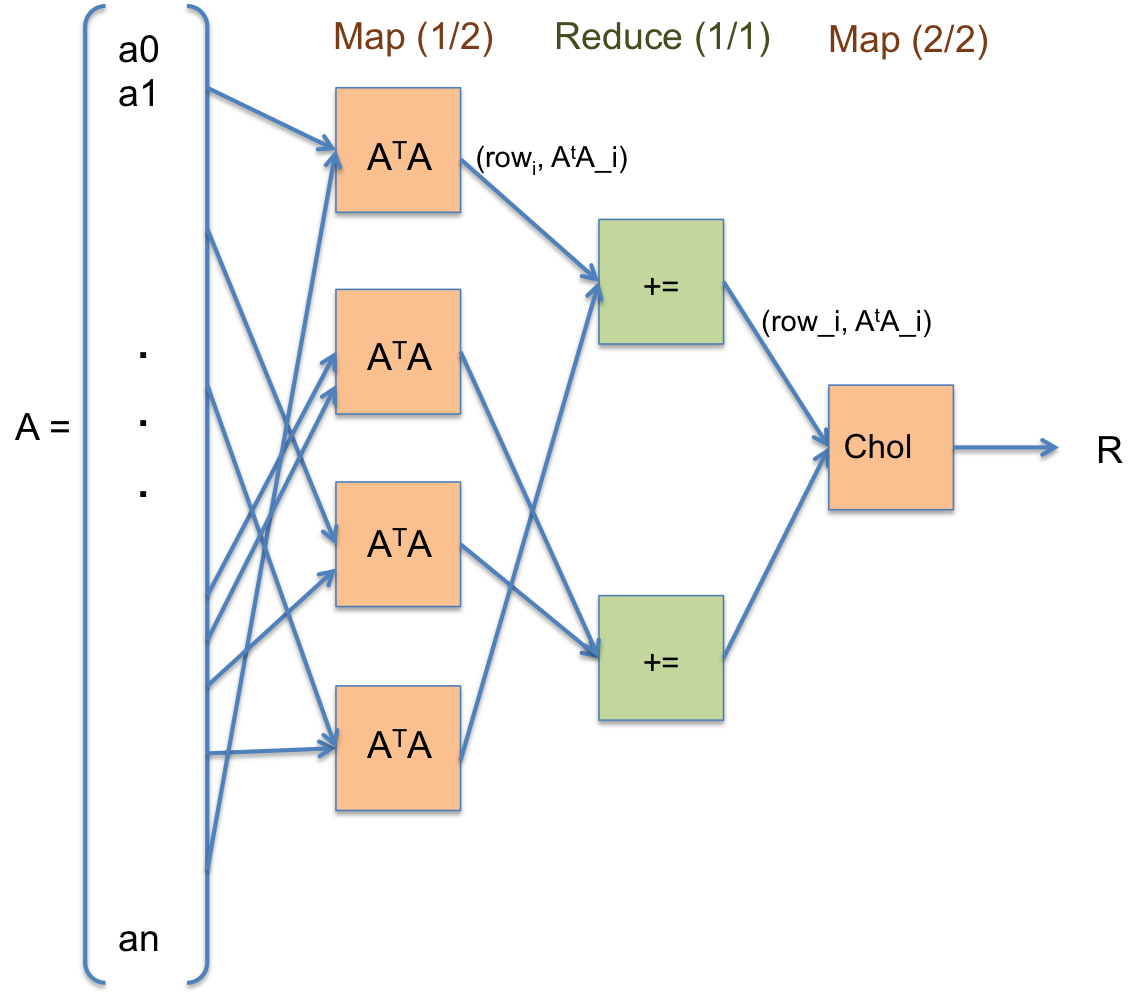
\includegraphics[height=2.5in]{./images/mrcqr.png}
\end{center}

\end{frame}

\begin{frame}
\frametitle{Mapper implementation}

Which of these implementations is better?

\vspace{0.2in}
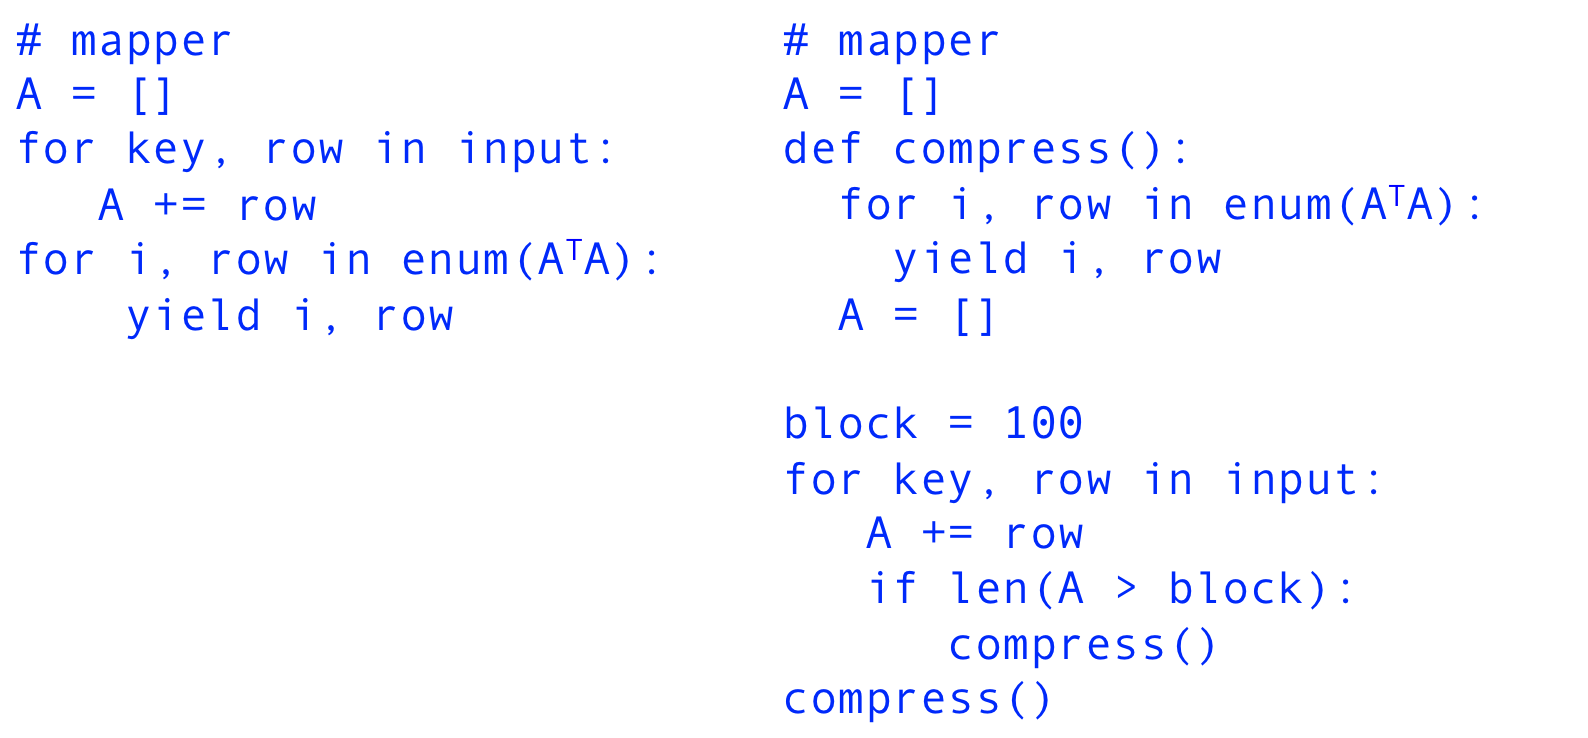
\includegraphics[height=2.in]{./images/chol_map1.png}

\end{frame}


\begin{frame}
\frametitle{Example: Cholesky QR}
\frametitle{Mapper implementation}

Which of these implementations is better?

\vspace{0.2in}
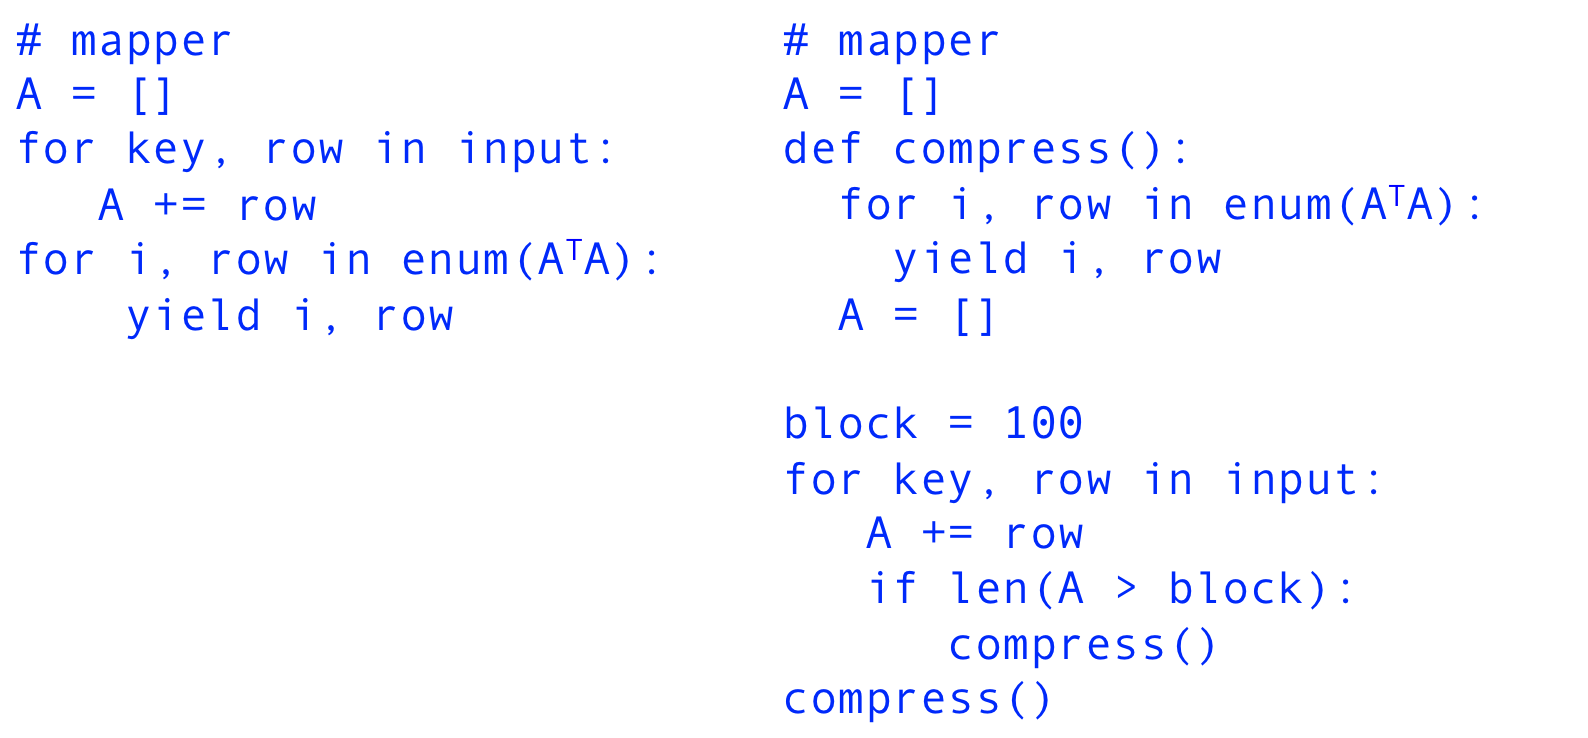
\includegraphics[height=2.in]{./images/chol_map1.png}
\vspace{0.2in}

Answer: the one on the left (usually)

\end{frame}

\begin{frame}

Why?

\vspace{0.4in}

\begin{enumerate}
\item{Shuffle time}
\item{Reduce bottleneck}
\end{enumerate}

\vspace{0.4in}

However, the left implementation could run out of memory.

\end{frame}


\begin{frame}
\frametitle{Mapper implementation}

Can we do better? Yes

\begin{center}
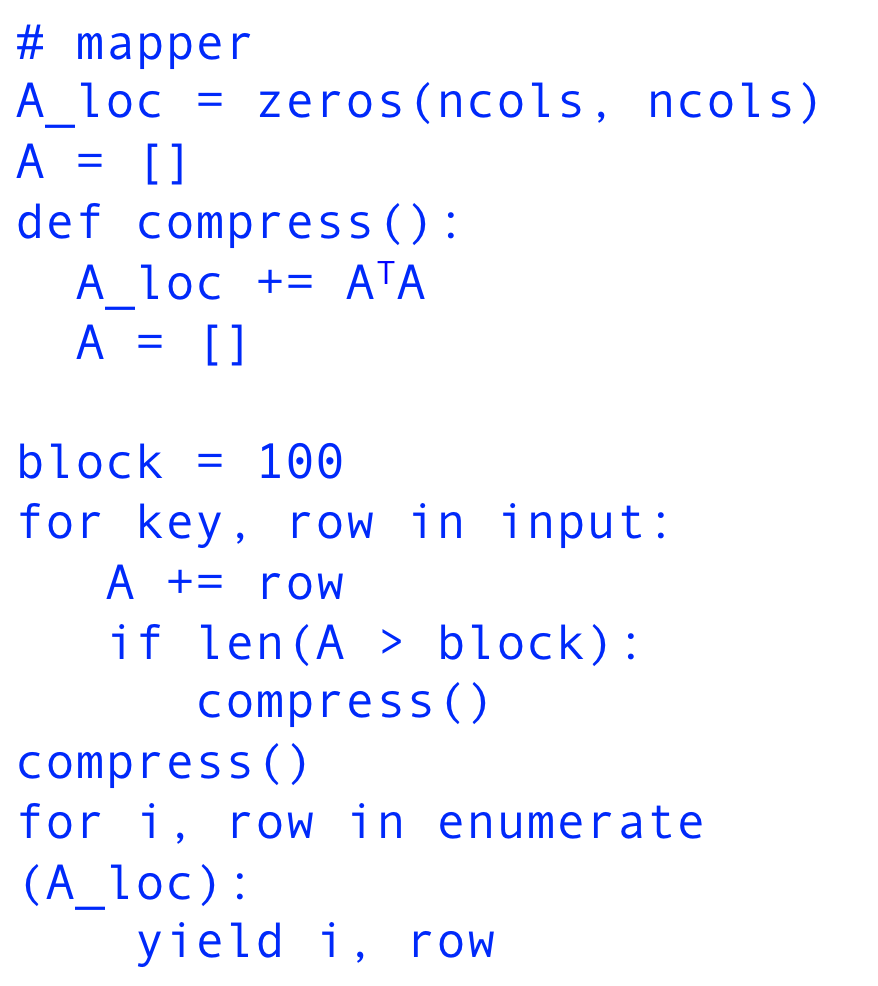
\includegraphics[height=2.5in]{./images/chol_map2.png}
\end{center}

\end{frame}


\begin{frame}

\begin{center}
Questions?
\end{center}

\begin{center}
\huge{Austin R. Benson \\
arbenson@gmail.com \\
https://github.com/arbenson/mrtsqr}
\end{center}


\end{frame}


\end{document}
